\begin{myprop}
	\begin{itemize}
		\iftoggle{eleve}{%
			\item Dans un triangle \hrulefill 
			
			\vspace*{0.2cm}
			\hrulefill 
			
			\vspace*{0.2cm}
			\hrulefill 
			
			\item Si la longueur \hrulefill 
			
			\vspace*{0.2cm}
			\hrulefill 
			
			\vspace*{0.2cm}
			\hrulefill 
		}{%
			\item Dans un triangle la longueur d'un coté est \kw{inférieure à la somme} des longueurs des deux autres côtés.
			
			\item Si la longueur du plus grand coté est égale à la somme des deux autres, le triangle est \kw{plat}.
		}
		
	\end{itemize}
	
\end{myprop}

\begin{mymeth}
	\iftoggle{eleve}{%
		\hrulefill 
		
		\vspace*{0.2cm}
		\hrulefill 
		
		\vspace*{0.2cm}
		\hrulefill 
		
		\vspace*{0.2cm}
		\hrulefill 
	}{%
		Pour vérifier qu'un \kw{triangle est constructible}, on vérifie que la longueur du plus grand côté  est inférieure à la somme des deux autres.
	}
	
\end{mymeth}

\iftoggle{eleve}{%
	%\newpage
\begin{myexs}
	
		
		\begin{multicols}{2}
			\begin{itemize}
				\item Le triangle ABC \hrulefill
				
				\vspace*{0.2cm}
				\hrulefill
				%\item Un triangle de cotés 8 cm, 5 cm et 6 cm est constructible (8 < 11).
				
				\item Le triangle $DEF$, \hrulefill
				
				\vspace*{0.2cm}
				\hrulefill
				
				\vspace*{0.2cm}
				\hrulefill
				
				\vspace*{0.2cm}
				\hrulefill
				
				\item Un triangle de coté 10 cm, 4 cm et 5 cm \hrulefill
				
				\vspace*{0.2cm}
				\hrulefill
				
%				\vspace*{0.2cm}
%				\hrulefill
				
				
			\end{itemize}
			
			
			\begin{center}
				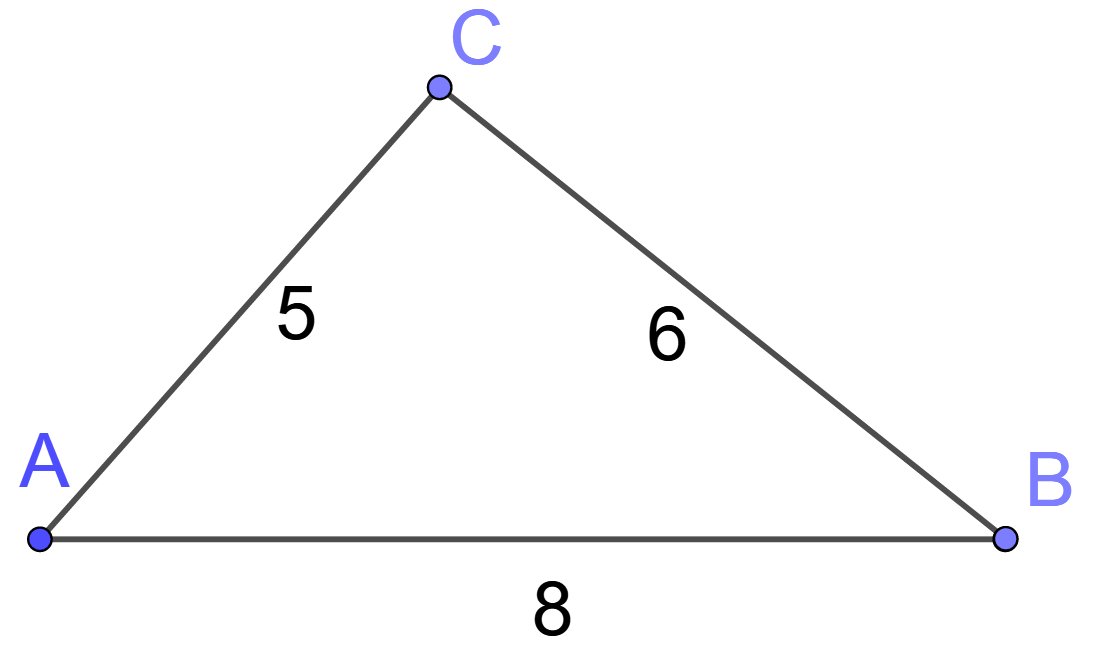
\includegraphics[scale=0.25]{triangle1}
				
				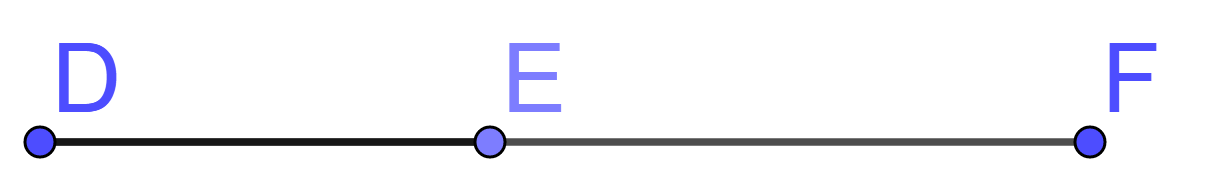
\includegraphics[scale=0.2]{triangle2}
			\end{center}
		\end{multicols}
	\end{myexs}
	}{%
	\begin{myexs}
		\begin{multicols}{2}
			\begin{itemize}
				\item Le triangle ABC est constructible, on a $AB < AC + CB$ (8 < 11).
				
				\item Le triangle $DEF$, tel que $DE = 7$ cm, $DF = 3$ cm et $FE = 4$ cm est plat, les points sont alignés ($4 + 3 = 7$).
				
				\item Un triangle de coté 10 cm, 4 cm et 5 cm n'est pas constructible ($10 > 4 + 5$).
			\end{itemize}
			
			
			\begin{center}
				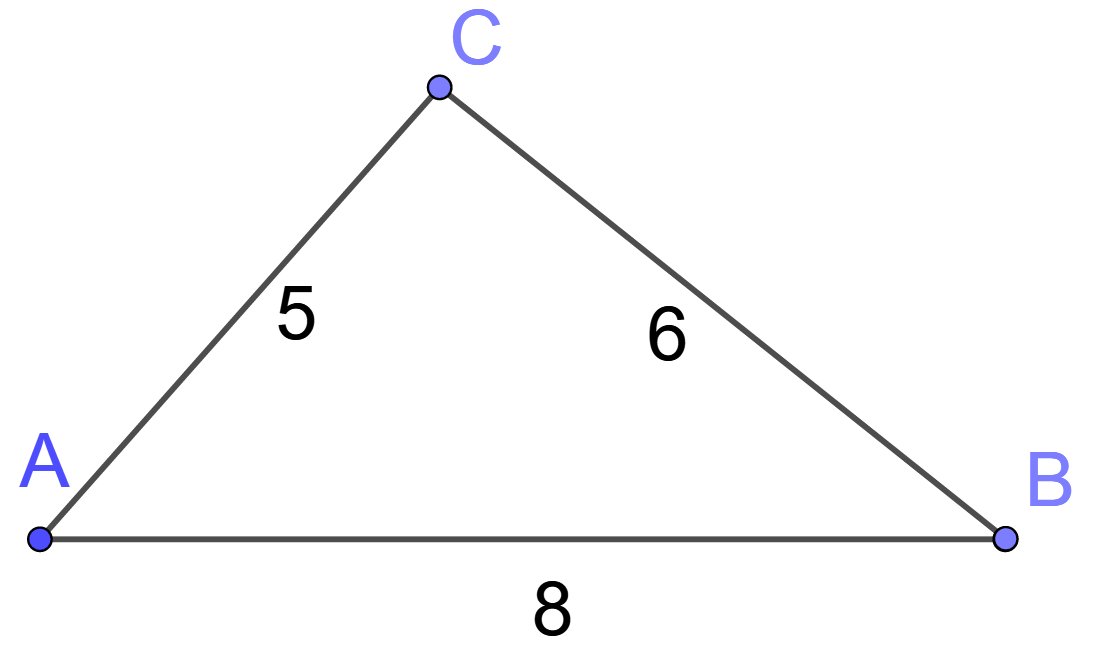
\includegraphics[scale=0.25]{triangle1}
				
				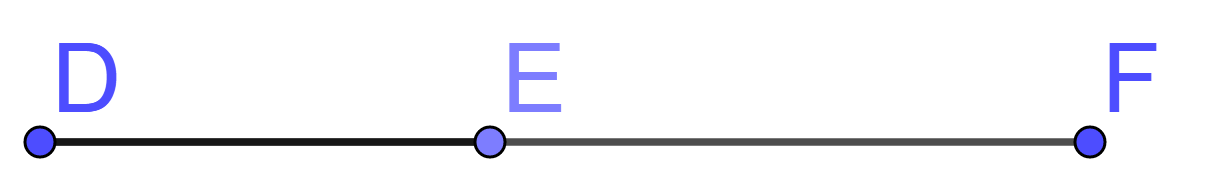
\includegraphics[scale=0.2]{triangle2}
			\end{center}
		\end{multicols}
	
	
\end{myexs}
}
